The objective of the control module is to be capable of, with an input reference velocity and steering angle, outputting the appropriate command variables to achieve said references. The first step in its design is to conceptualize the car's model; since the interest lies in the motion of the car, the kinematic model will be the one to be studied.
\subsubsection{Conception Of Car Model}
\label{sec:concep}

\begin{figure}[!htbp]
\centering
       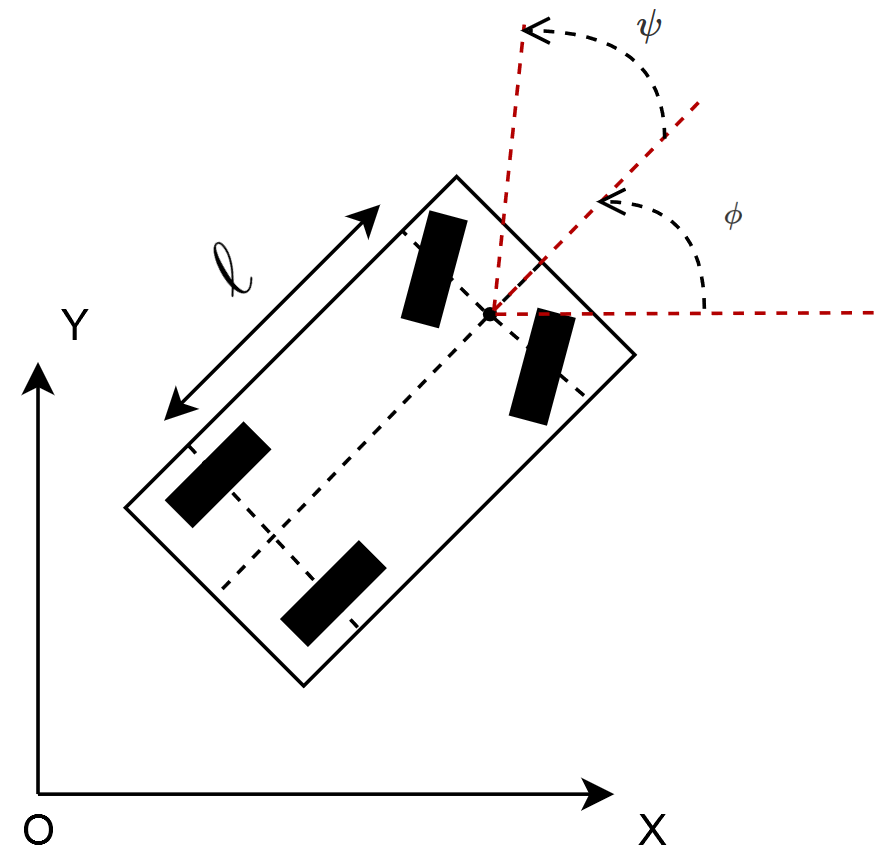
\includegraphics[page=1,width=0.6\textwidth]{img/kinematicModel.png} 
\caption{Kinematic Model of Car}
\label{fig:kinModel}
\end{figure}

Considering the kinematic model of a four-wheel vehicle with a wheelbase length $\ell$, a linear velocity v(t) and an angular velocity $\omega(t)$ the following situation will occur: since the rear wheels will remain in the same position no matter where the car is facing towards, they will be facing whatever orientation, $\phi$, the car is facing, however, in order for the car to be capable of moving into wherever the user tells it to, the front wheels must turn, ergo a steering angle $\psi$, must be considered. The resulting direction the car will be going in is $\phi + \psi$. With these considerations, a desired angle of tilt $\theta$ and considering that $\phi=0$, in other words, that whatever direction the car is told to face, it will be relative to its current direction, the following model is obtained:
\begin{align}
\dot{x}&=v(t) cos(\psi)\\
\dot{y}&=v(t) sin(\psi)\\
\dot{\psi}&=\omega(t)=\frac{v(t)}{\ell}\theta
\end{align}
However this model is not enough for simulation purposes. The simulation has the objective of granting the designers clear ideas of the response of the systems towards given inputs, therefore, for implementation purposes, the simulation must give feedback on the position of the car, its heading and the linear velocity of the right rear wheel ($v_r$), and the left rear wheel ($v_l$) therefore the model will have to changed with these details in mind, which can be achieved considering that:
\begin{align}
\omega(t)&=\frac{v_r(t)-v_l(t)}{\ell}\\
v(t)&=\frac{1}{2}(v_r(t)+v_l(t))
\end{align}
Solving the system above for $v_r$ and $v_l$:
\begin{align}
v_ r(t)&=v(t)+ \frac{\omega(t)\ell}{2}\\
v_l(t)&=v(t)-\frac{\omega(t)\ell}{2}
\end{align}
Returning the model in order to $\dot{x}$ and $ \dot{y}$:
\begin{align}
\dot{x}&=v(t) cos(\psi)-\frac{\ell}{2}\omega(t) sin(\psi)\\
\dot{y}&=v(t) sin(\psi)+\frac{\ell}{2}\omega(t) cos(\psi)\\
\dot{\psi}&=\omega(t)=\frac{v(t)}{\ell}\theta
\end{align}
\subsubsection{Simulation Model}
The mathematical model determined in Section~\ref{sec:concep} was simulated in
the Matlab/Simulink environment. Converting the mathematical model into a
simulink subsystem yields (Fig.~\ref{fig:carModel}):
\begin{figure}[!htbp]
\centering
       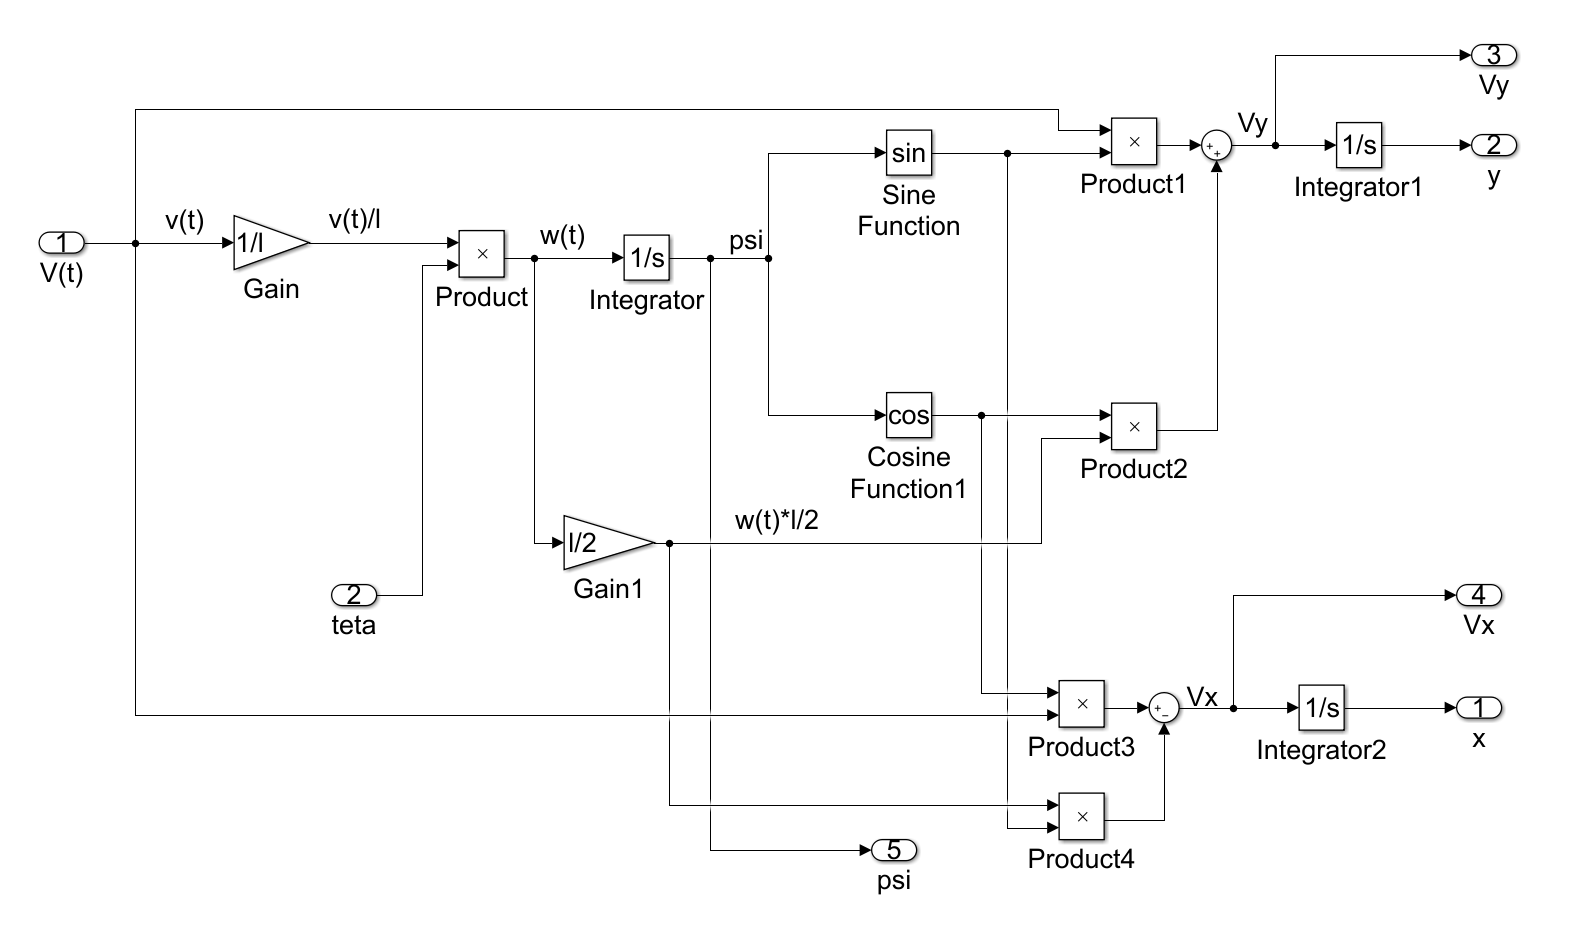
\includegraphics[page=1,width=1\textwidth]{img/subsystem.png} 
\caption{Car Model in a Simulink Subsystem}%
\label{fig:carModel}
\end{figure}
After obtaining the model of the car, the control simulations of the system may begin:
\begin{figure}[!htbp]
\centering
       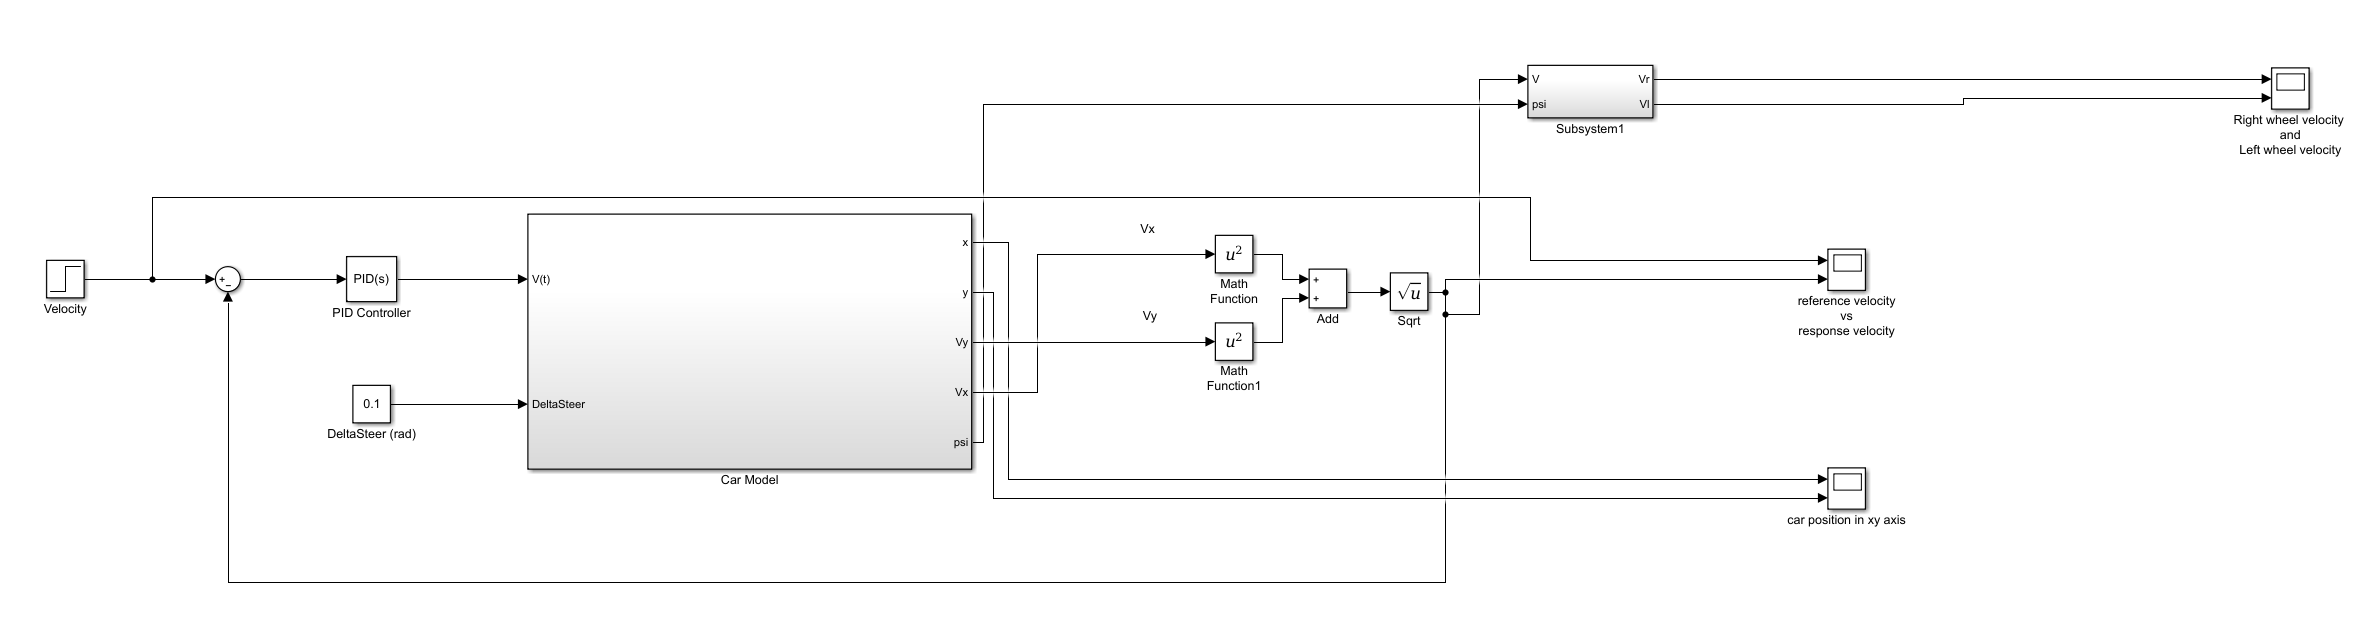
\includegraphics[page=1,width=1\textwidth]{img/system.png} 
\caption{Simulation Schematic}
\end{figure}\\
The simulation schematic uses the model in Fig.~\ref{fig:carModel} within the
`Car Model' subsystem to simulate the response of the system to a step reference
of the desired velocity and a constant reference of the angle to which the car
should turn towards. It calculates the norm of the velocity vector, returns it
as feedback and also uses it to pass through subsystem1 that will return the
different velocities at which each of the rear wheels must turn in order to
achieve said angle.
%%% Local Variables:
%%% mode: latex
%%% TeX-master: "../../../dissertation"
%%% End:
